% -*- root: rapport.tex -*-
\documentclass[a4paper, 12pt]{article}
\usepackage{graphicx}
\DeclareGraphicsExtensions{.pdf,.png,.jpg}
\usepackage{xcolor}   %May be necessary if you want to color links
\usepackage{hyperref}
\usepackage{mathtools}
\usepackage{listings}
\usepackage{pgfplots}
\usepackage{pgfplotstable}
\usepackage{booktabs}
\usepackage{wrapfig}
\usepackage{csquotes}
%\usepackage{inconsolata}




\hypersetup{
    colorlinks=true, %set true if you want colored links
    linktoc=all,     %set to all if you want both sections and subsections linked
    citecolor=black,
    filecolor=black,
    linkcolor=black,
    urlcolor=blue
}

\lstdefinestyle{customc}{
  belowcaptionskip=1\baselineskip,
  breaklines=true,
  frame=single,
  language=C,
  showstringspaces=false,
  basicstyle=\footnotesize\ttfamily,
  keywordstyle=\bfseries\color{green!40!black},
  commentstyle=\itshape\color{purple!40!black},
  identifierstyle=\color{blue},
  stringstyle=\color{orange},
  tabsize=4
}
\lstset{escapechar=@,style=customc}

\title{Utilizing Amazon's Zookeeper to handle scaling and maintenance of a Voldemort cluster}
\author{Eivind Siqveland Larsen and Knut Nygaard,\\
        Department of Computer Science,\\
        NTNU,
        Trondheim}

\begin{document}
\maketitle
\thispagestyle{empty}

\clearpage


\begin{abstract}
NoSQL databases often support scalability and high availability.
We address Voldemort, which is a popular, highly available NoSQL database that can be run on several nodes.
The system is cumbersome to setup and maintain. As clusters grow in size, scaling into hundreds of nodes, management and administrative tasks become increasingly complex. We have therefore focused on automating management of a running cluster of nodes.

We have migrated the configuration storage of the Voldemort distributed NoSQL database from local XML files on disk to global objects using Apache ZooKeeper.

Using native tools and ZooKeeper coordination, we have implemented a fault tolerant, redundant service. The service manages node discovery, configuration generation and propagation. It also has components for live monitoring and adjustment of responsibility to match each nodes available system resources.

\end{abstract}

\clearpage
\renewcommand{\abstractname}{Sammendrag}
\begin{abstract}
Vi har flyttet konfigurasjon av en distribuert NoSql database fra lokalt lagrede XML filer til globalt tilgjengelige objekter ved hjelp av Apache ZooKeeper.

Vi har brukt ZooKeepers egenskaper for koordinasjon og andre verktøy til å implementere en feiltolerant, redundant tjeneste for å ta hånd om nye noder, generere konfigurasjonsfiler, propagere endringer og automatisk tilpassing av det kjørende systemet til den enkelte nodes tilgjengelige systemressurser.
\end{abstract}

\clearpage


\begin{aknowledgements}
We would like to than Svein Erik Bratsberg for his guidance and assistance in the project.
We would also like to thank LinkedIn for creating and publishing their take on Dynamo and making it open source.
\end{aknowledgements}

\clearpage

\tableofcontents
\clearpage

\listoffigures
\clearpage
\setcounter{page}{1}

% introduction.tex

\section{Introduction}
This section explains the background for our project, what goals we have and what methods we have employed to reach our goals. 

Section \ref{sec:technical_background} explains technology and techniques commonly used in distributed systems.

TODO: INTRODUCE OTHER SECTIONS AND CHAPTERS

\subsection{WHAT}
Short what and why.

We have chosen to work with Voldemort, which is an open source implementation of Amazon’s Dynamo. 


\subsection{Background}
Traditional relational database systems are generally very safe to use, usually providing all of the ACID (\emph{Atomicity, Consistency, Isolation, Durability}) properties.
This guarantees that all committed transactions are processed reliably. 
Today a lot of services needs to support up to millions of users and serve thousands of requests per second, but experience has shown that databases providing ACID guarantees have trouble scaling. 
To allow for cost effective scaling commodity hardware is used instead of expensive specialized servers. To continue scaling by adding numerous small servers, applications need to become increasingly distributed.

The main reason for ACID databases having troubles scaling is the strong guarantees of atomic operations, isolation and consistency. 
To allow for atomic operations in a distributed systems a distributed commit log would be required. 
Similarly to guarantee isolation distributed locks would be required. In a system with thousands of concurrent users lock contention can become a serious issue. 
Lastly to guarantee consistency across multiple machines requires significant overhead with regards to keeping all replicas consistent. 

Distributed NoSQL databases often sacrifice consistency and isolation requirements to achieve higher availability with satisfactory durability. These systems often provide a highly available service and eventual consistency.
The databases are designed to scale linearly, however managing and scaling these systems are not always trivial\cite{tellybug}. 


\subsection{Voldemort and Dynamo}
Voldemort is a distributed key-value storage system based off Amazon's paper on Dynamo, Amazons's highly available key-value store. Voldemort was created by LinkedIn and the first public release was in 2009. It is still under development. Voldemort supports a simple set of operations limited to put, get and delete. Stored objects are uniquely identified by a key and are considered by the system as binary blobs. Voldemort is commonly used for storing lots of smaller objects, typically less than 1MB.  As with other NoSQL implementations, Voldemort sacrifices consistency and isolation requirements to achieve higher availability with satisfactory durability. In fact, we will later see that most of this behavior is easily tunable and left as design choices per implementation.

Compared with Apaches Cassandra, Voldemort lacks the power of column families and multi-key lookup. This means that any application powered by Voldemort requires addtional logic to handle more advanced queries. For simple read heavy workloads however, Voldemort is blazingly fast serving over 20 000 read requests per second per node. 

Voldemort is currently being used by a number of known companies. At LinkedIn they use Voldemort both as read-only and read-write stores. Services powered include LinkedIn Search, news and Who viewed your profile. At Ebay they use Voldemort as a read-only store for distributed lookups, and the dating site eHarmony uses Voldemort as a high volume read/write store.

There are several factors that was important for us when choosing which distributed key-value store to work with. We both had detailed theoretical knowledge of Dynamo after holding a presentation on their paper. The simple design and data model of Voldemort also was a good fit for our project as we did not have any application specific requirements for our storage system to meet. Lastly we wanted to work with an open source project. Voldemort fulfilled all these requirements. 

Voldemort keep its configuration data in several XML files. These files reside on each individual node in the cluster. The process of executing a repartition or rebalance involves another set of xml files as well as various scripts that must be run. As the number of nodes grows this number of configuration files can get out of hand quickly. 
As a result, creating a system to handle these configuration files was proposed as a ``fun project'' on the project-voldemort website. Apache ZooKeeper was proposed as a possible service for this system.  


\subsection{Goals}
We have chosen to implement this proposed configuration system by moving Voldemort's configuration data into ZooKeeper. In addition we would like to utilize the powerful features of ZooKeeper to create an automated service for managing a running Voldemort cluster. 

% Create a system for automatically including new nodes in a set of member nodes.
% For Voldemort, this includes redistributing partitions and updating routing information without making the system unresponsive, i.e. without incurring downtime.

In short our goals are the following:

\begin{enumerate}
	\item{Move Voldemort configuration data away from each local node and into ZooKeeper}
	\item{Simplify the rebalance process using ZooKeeper}
	\item{Create a service for automatic management of the cluster, including node discovery, membership and rebalancing with new members}
	\item{Create a monitor service to monitor live nodes}
\end{enumerate}

\subsection{Method}
We plan to use virtual machines as our cluster nodes. This greatly simplifies setup of environments and scaling, but is not ideal for performance. We will rewrite the MetadataStore in Voldemort to utilize ZooKeeper instead of local files. As ZooKeeper does not offer advanced primitives, we need to write the ones we need. Finally we will create a service for node discovery, membership and automatic management. The monitor service will act as decision support system for this automated service. 


% The supported queries are limited to simple get and put operations on objects uniquely identified by a key. 
% The objects stored are by the system considered binary blobs.
% The database is mainly used to store lots of smaller items, typically less than 1MB in size.

% Voldemort and Dynamo sacrifices consistency and isolation requirements to achieve higher availability with satisfactory durability.
% In fact, we will later see that most of this behavior is easily tunable and left as design choices per implementation.
% You should also note Voldemort (and Dynamo) does not guarantee any form of isolation and does not support multiple key updates.


%\subsubsection{Motivation for these systems}
%Traditional relational database systems are generally very safe to use, usually providing all of the ACID (\emph{Atomicity, Consistency, Isolation, Durability}) properties.
%This guarantees that all committed transactions are processed reliably.
%Experience has however shown that databases providing ACID guarantees have trouble scaling. It is very difficult, if not impossible, to have ACID databases handle the high traffic volumes in addition to the high availability demands of today.

%Voldemort and Dynamo sacrifices consistency and isolation requirements to achieve higher availability with satisfactory durability.
%In fact, we will later see that most of this behavior is easily tunable and left as design choices per implementation.
%You should also note Voldemort (and Dynamo) does not guarantee any form of isolation and does not support multiple key updates.



\clearpage

\section{Related work}
In this section we will cover Cassandra and HBase. Two other distributed systems that are used 

\subsection{Cassandra}
Cassandra scalable NoSQL database now available as open source through the Apache foundation. It was built from scratch with goal of being a massively scalable NoSQL database. In a cluster running Cassandra there is no sense of a master node, and all communication between nodes use peer to peer and the gossip protocol. As an administrator it is easy to scale Cassandra to meet both current and future system requirements. 

\subsubsection{Reads and writes}
In Cassandra all participating nodes can be accessed for writes and reads. To ensure durability all writes are preceded by a write to a commit log. If a node has crashed, a node holding a replica will service reads and writes according to the hinted handoff strategy. As with Voldemort, Cassandra also features tunable consistency. 

\subsubsection{Data model}
The Cassandra data model is based on a key:value model, however Cassandra extends this model with up to two levels of nesting. This forms a map structure called columns where the outer row key acts as a primary key and the inner sorted map holds all information: \texttt{Map<RowKey, SortedMap<ColumnKey, ColumnValue>>}. By using maps we achieve easy lookups and range scans. By using one more level of nesting we can group columns. These are called super columns. In Cassandra de-normalization is used to be able to efficiently perform queries that accesses information stored in separate columns. To allow this composite columns can be created to match the need of one or more specific queries. These composite columns simply gather information already stored in various columns for easier access. 

\begin{figure}[h]
    \centering
    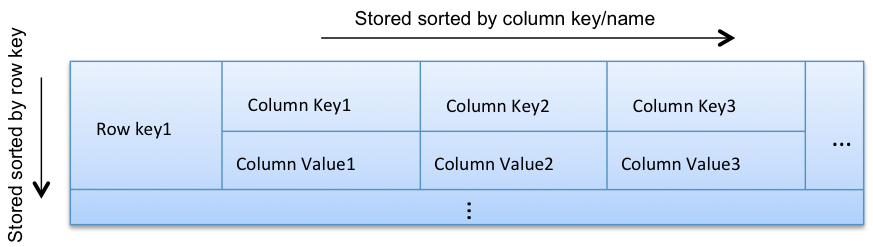
\includegraphics[width=0.5\textwidth]{resources/cas_col.png}
    \caption{A sample column. The row key acts as a primary key and each key:value pair would hold one field in a table. Images borrowed from www.ebaytechblog.com}
    \label{fig:sample_col}
\end{figure}

\begin{figure}[h]
    \centering
    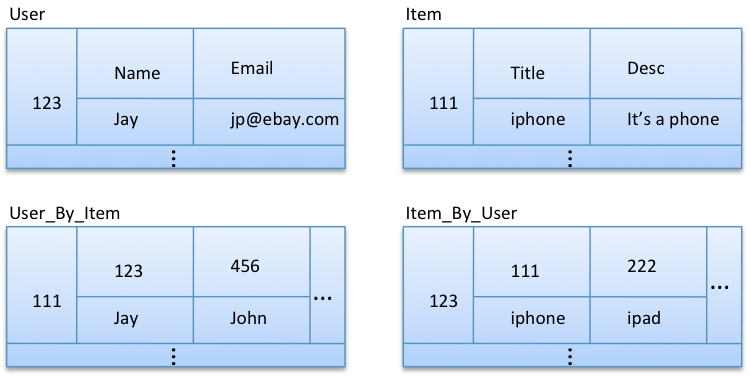
\includegraphics[width=0.6\textwidth]{resources/cas_comp_col.png}
    \caption{A sample composite columns. Here we have separate composite column to efficiently be able to serve queries on users by item and item by users.}
    \label{fig:sample_comp_col}
\end{figure}

\begin{figure}[ht]
	\centering
	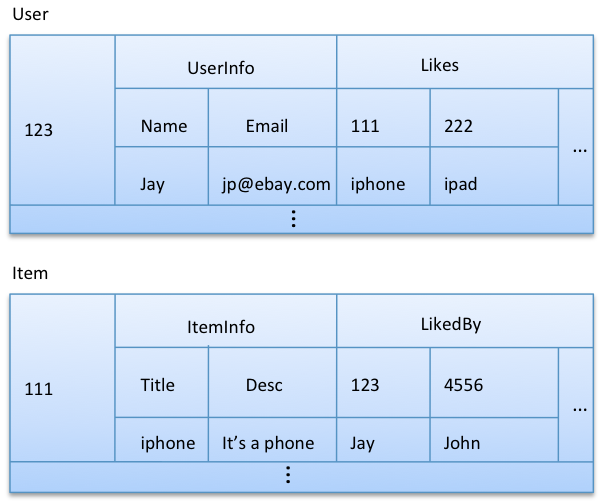
\includegraphics[width=0.4\textwidth]{resources/cas_super_col.png}
	\caption{A sample super column. Here we can see an outer map containing a person and the inner maps consisting of various composite columns}
	\label{fig:sample_super_col}
\end{figure}

Cassandra is used by several well known companies. Netflix uses Cassandra for several applications, including its subscriber system and viewer history service. Facebook used Cassandra to power their inbox search, however this was abandoned in late 2010 in favor of HBase. Spotify also migrated to Cassandra after migrating away from postgreSQL because of scaling issues. They use Cassandra to store playlists, radio stations and notification notifications.

\subsection{HBase}
HBase is based on Googles paper on BigTable.
It is a sparse, distributed, persistent multi-dimensional sorted map.

With regards to the CAP-theorem (Consistency, Availability, Partitioning), HBase provides consistency and tolerance to partitioning, making HBase fault tolerant and easy to reason with in practice.

Important to note is that HBase provides a sparse multi-dimensional \emph{sorted} map.
Keys in the table are sorted, such that similar items are close to another when scanning a table.

E.g. when storing data about urls, the keys are written in reverse: \texttt{com.google.www/users}. This scheme keeps urls from the same domain and subdomain close to each other in the sorted map.

The \emph{rows} or \emph{entries} are typically sparse, meaning that most of the columns, in the table are empty.

To visualize a HBase record, it can help to think of a map of maps:

\begin{lstlisting}
{
	"com.google.www/account": {
		"family": {
			"special": "value"
		},
		"anchor": {
			"com.cnn.www": "value"
		}
	}
	"com.google.www/users": {
		"family": {
			"": "value"
		},
		"anchor": {
			"no.nrk.www": "value"
		}
	}
}
\end{lstlisting}

The families for a record is static for the table at creation, but every family can hold any number of columns within, even many or none.
This is where the sparse property comes from, as most entries will not have a value for the set of all sub-families in the table, leaving most column values empty.

Every \emph{row} or \emph{entry} also has an associated timestamp, used for versioning. This is typically a monotonically increasing number, such as seconds since \emph{epoch}. HBase stores a given number of versions of an entry, and can be queried for these. 
These different versions are stored in descending order, such that the highest number entry, i.e. the newest, is the first entry.

This gives a possible query structure as such \texttt{<key, family:column, timestamp>}. Timestamp is optional. If no timestamp is given, the newest entry is returned. 
If the query has a timestamp, the record with version equal to or less than the given timestamp is returned. If there is no such record, null is returned.

I.e. if we have a query \texttt{<no.nrk.www, referrals:no.nrkbeta.www, 999>}, and we have records in the database:
\begin{lstlisting}
<no.nrk.www, referrals:no.nrkbeta.www, 1001>
<no.nrk.www, referrals:no.nrkbeta.www, 777>
\end{lstlisting}
\texttt{<no.nrk.www, referrals:no.nrkbeta.www, 777>} will be returned.

\subsection{Bone dry servey that explains performance}

\subsection{Netflix Priam for Cassandra}

\subsection{Autoscaling Cassandra clusters}

Baakind\cite{baakind} created a system, called Hecuba, for automatic expansion of Cassandra clusters.

The goal of the project is an automatic scaler for Cassandra. The scaler should based on resource usage be able to increase or decrease the cluster size, based on resource usage in each node of the cluster.
The scaler should not affect the performance of Cassandra. This includes the overall operational capacity for the cluster, as well as only executing scaling when the cluster can handle it, i.e. during times of lower load.

Hecuba includes a master service, which collects information from all the nodes in the cluster, and tries to keep a view of the current status. The Cassandra nodes periodically sends status reports to the master, e.g. one every second. The status report includes size of database, CPU load and memory usage. The master is configured with certain parameters for what loads are allowed, such as maximum memory and CPU load over \emph{a given period of time}.

Like Netflix' Priam, Hecuba does scaling if a threshold is broken for a given period of time. Let's assume a CPU load of 60\%, threshold 55\%, and a period of 10 seconds. Hecuba will then only scale if the CPU load is reported as greater than \emph{threshold} for at least 10 seconds in a row.


\clearpage


\section{Technical background}
\label{sec:technical_background}

The software used in this project employ many different and important techniques known from distributed computing, which will be discussed here.
In section \ref{sec:consistenthashing} we will talk about the key aspect consistent hashing.
We will then discuss how consistent hashing techniques help us build \emph{available} and \emph{durable} databases.

Section \ref{sec:failures} discusses how failures are handled in the system. The tunability of the database is introduced in section \ref{sec:tunability}.

We lastly introduce PAXOS, a protocol for reaching consensus in a set of independent nodes.

\subsection{Consistent hashing}
\label{sec:consistenthashing}
Consistent hashing is a technique introduced in 1997 by David Karger\cite{Karger97consistenthashing} et al.
The technique is used to solve problems with locating a key in a distributed system.
Assume you have $n$ servers in the system, then number these from $0$ to $n-1$.
The \emph{hashspace} of the keys are then divided into $n$ partitions. Then, to find which server to put a key on, do a $$\textrm{Hash(key) mod } n$$ and you have the server number for the key. 

However, with this scheme if a server fails and you now have $n-1=m$ servers, all the failed server's data is gone.
You have to invalidate all existing servers, renumber your set of servers and start over.
Analogously, if you add $k$ servers to accommodate higher traffic, you now have $$\textrm{Hash(key) mod } n + k$$ and it is easy to see that all or most keys will have to relocate.

Consistent hashing reduces this problem by assigning each node with a number of points in the hash space.
The hash space is viewed as a ring by wrapping around \texttt{0000-FFFF}. The nodes are placed at points along the ring as in Figure \ref{fig:hashring}. When a key is looked up, you find it's place on the ring and move clockwise to the first point with an assigned node. In Figure \ref{fig:hashring}, key K is routed to the next node on the ring, node B.

Now remember we let the nodes take on \emph{several} points along the ring, thus spreading a nodes responsible key space to smaller pieces along the ring.
I.e. nodes B, E and G in Figure \ref{fig:hashring} could be the same \emph{physical} node.

\begin{figure}[h]
    \centering
    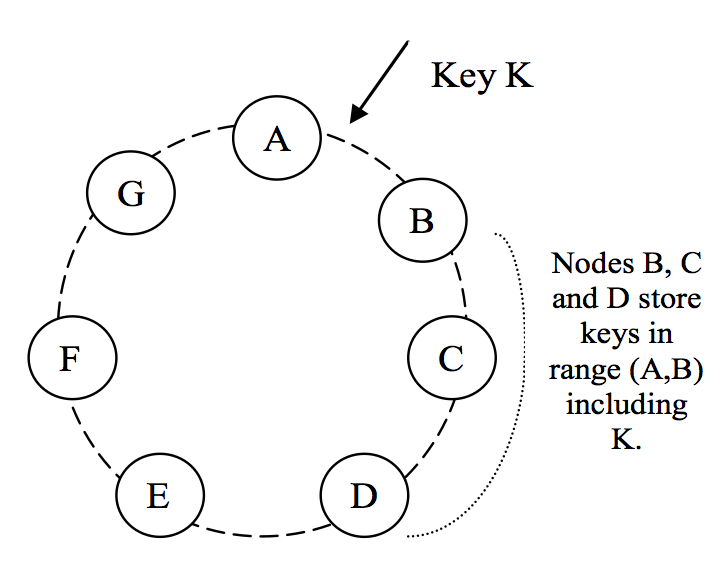
\includegraphics[width=0.5\textwidth]{background/figures/hashring}
    \caption{Hash ring with several nodes\cite{dynamo}.}
    \label{fig:hashring}
\end{figure}

This approach to locating keys has several advantages:

\begin{itemize}
\item Like before, we distribute operations on the set of available servers. By having each server take numerous positions on the hash ring, we also gain a more even distribution of the amount of key space among the nodes, compared to giving them a single random or fixed position.

\item Consistent hashing can also accommodate different types of servers by allowing more powerful nodes to have more points assigned on the ring, and vice versa. 

\item When adding a new server, a number of different areas around the circle are affected, and not one contiguous piece. This means the work of adding in the new node will be spread over the system, and not all requests routed to a single node.

\item The spread of the key space also avoids rehashing of more than $k/n$ keys when adding a new node. 

\item When a node fails, you move along the ring to the next server. When the nodes occupy several points on the ring, the extra work because of a failing node will be distributed among all the nodes in the system.
\end{itemize}

Consistent hashing also conveniently allows for easy, tunable replication of data to ensure durability, as used by key-value stores Dynamo\cite{dynamo} and Voldemort\cite{voldemort}. Consider W the number of data replicas to create. Hash the key, then move along the ring, writing key K to the W first nodes encountered on the ring. This will also ensure backups to be available along the ring when a node fails and requests gets passed along.

\subsection{Durability}
As explained in \ref{sec:consistenthashing}, both Voldemort and Dynamo use consistent hashing to locate and store keys.
They are both key-value stores only.
The goals for the Voldemort project is a database which is highly available and fault tolerant, providing an \emph{always-on} experience.

To safely store user data, redundancy is required. 
The typical approach to this is synchronously storing replicas at different locations to ensure data replication. 
In practice though, providing this kind of strong consistency in a database system can prove detrimental to availability in some failure scenarios.
A common approach to failure is locking down data and making it unavailable until the failure is resolved, so as not to serve potentially stale or erroneous data.
While it is convenient for the programmer to never have to deal with possibly failed data, locking down doubtful data is not ideal for performance.
In distributed systems network and system failures can be quite common, making guarantees of strong consistency very costly. In practice, strong consistency can be considered incompatible with high availability.
This makes traditional replication methods unsuitable for highly concurrent distributed systems.

\begin{wrapfigure}{R}{0.5\textwidth}
    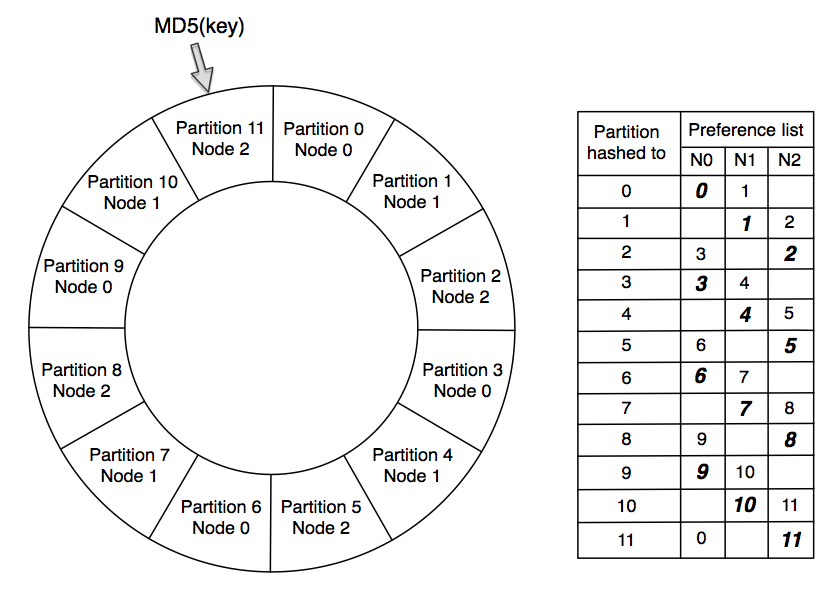
\includegraphics[width=0.5\textwidth]{background/figures/hashring_voldemort}
    \caption{Hash ring with 3 nodes and 12 partitions from Voldemort\cite{dynamo} with N=2. Partitions are a fixed number of splits of the keyspace. Nodes are assigned a number of partitions which they hold. When a request is routed, one first hashes the key to find the partition the key belongs on. One then asks nodes in the order of the \emph{preference list} for the key.}
    \label{fig:voldemort_hashring}
\end{wrapfigure}

To help provide higher availability of data, an optimistic approach to replication is used.
By allowing replicas to gradually propagate in the background and not synchronously, the workload on a distributed database system is greatly relieved, allowing for higher throughput. By also allowing conflicting data, we can continue to serve data in times of failure. This will cause more work for the application developers, and they need to be aware of this when using the database. Allowing conflicts also helps availability of put operations, and allows us the possibility to always accept a write.

It is easy to see how the consistent hashing ring helps implement this approach in Voldemort.
To ensure data durability, one can simply write the data to the next few nodes on the ring. In Dynamo and Voldemort this is a tunable parameter, W, which controls how many nodes a write synchronously has to reach to be successful. 
Internally it is called \emph{required writes}.

Similarly, it is easy to see how we can implement optimistic replication:
By allowing nodes to push written objects in the background, at a later time, to any number of nodes further down the ring.
This number \emph{N}, is called the \emph{replication factor}, and designates the number of replicas we \emph{eventually} want to be present.
I.e. we will have an \emph{eventually consistent} form of replication.

You should also note that this replication has two benefits: 
\begin{itemize}
	\item As a data backup should the other node have a hard drive failure.
	\item As a functional backup. If the other node is off line, the replica can take over the workload with all the data available.
\end{itemize}

In Voldemort, the hash ring is split into X equally sized parts, called \emph{partitions}. Each partition is assigned a unique ID and maps to a node.
The nodes create a \emph{preference list} over the partitions, which says to which \emph{partitions} it should store the replicas.

Now let $N=2$ with 12 partitions as in Figure \ref{fig:voldemort_hashring}. 
Let a key K's hash belong in partition 0. From the preference list, we see that this key should be put in \texttt{node0}, and replicated to the node holding partition 1, which is \texttt{node1}.
Voldemort also does some sanity checking when replicating, such that replicas are always replicated to N \emph{physical} nodes. 
I.e. In our example, if both partition 0 and 1 where held by \texttt{node0}, Voldemort would move along the ring until it finds the next partition that is assigned to a different node before storing the replica.

\subsection{Dealing with data conflicts}
Introducing optimistic replication to increase availability of the system, even in cases of nodes being unavailable for arbitrary reasons, has its price. 
In a distributed system nodes can be unreachable for a number of different reasons:
Network splits, nodes dying, overloaded network points and concurrent operations (remember no isolation or locking) may introduce conflicts in the data set.
These conflicts \emph{will} arise and need to be discovered and resolved at some point.

How to deal with conflict is an important decision.
The question of when to resolve them and who should have the responsibility of doing so all have different properties.
A traditional approach is to resolve conflicts when they appear, i.e. on writes. 
This has the benefit of keeping read logic simple, but we may have to reject a write if not all (or a majority of) replicas are reachable. Resolving conflicts on write is also easy for the user to reason with.

Voldemort however wishes to run an always writable store. No data write should fail, even during periods of network splits and failing nodes.
This requirement makes it impossible to resolve conflicts on write, and forces us to do conflict resolution on read.

This leaves the question of who should resolve the conflicts. We can either let the database store do conflict resolution or leave it to the application.
If the store itself is going to resolve conflicts, it's choices in doing so are relatively limited.
The store can not include domain knowledge for every possible application, so it can only do simple choices like last write wins or append the difference (which isn't even resolved, and probably destructive to the stored data). Recall that to the store most of the values are considered binary blobs.

The application however has intricate knowledge of the data and is in a much better position to make good decisions. 
Amazon\cite{dynamo} uses their shopping cart as an example. If two writes are two different products added to a shopping cart, we can record both of the writes even if they are divergent.
Then at read, the application can use both versions to create a new cart with both products in it, i.e. merge the changes in a reasonable way, and present them to the user.
This requires a bit of work from the developer, which they may not want or need to do, so there is also the option of doing simple conflict resolution on the server.

To be able to record all changes (writes), Voldemort uses a versioning system to record the history of all changes. The data are immutable blobs, and each write creates a new version with a history of predecessors.
To record this version history, Voldemort employs \emph{vector clocks}.

Roughly vector clocks are implemented as a list of \texttt{(node, counter)} pairs and this list is stored with every version of every stored object.
By evaluating the vector clocks between two versions (or more), we can decide if one is an ancestor of the other or not. If \texttt{A} followed as a version of \texttt{B}, we can discard \texttt{B} and use \texttt{A} because the changes for \texttt{B} are already included in A. 
If the histories are divergent, we have a conflict and need to do some sort of merge or resolution. More formally an object \texttt{A} is an ancestor of \texttt{B} if all the clocks in \texttt{A} are less than or equal to the clocks in \texttt{B}. 
If so, we can safely discard \texttt{A}.

%\begin{wrapfigure}{r}{0.5\textwidth}
\begin{figure}[h]
    \centering
    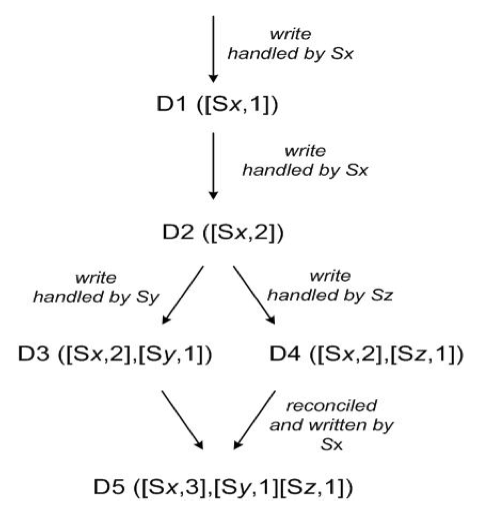
\includegraphics[width=0.7\textwidth]{background/figures/versioning}
    \caption{Version history for an object\cite{voldemort}.}
    \label{fig:versioning}
\end{figure}

To use vector clocks in this manner safely, it is required that all update operations (writes) specify which version we are updating, or we would not be able to infer causality.
This version information must first be obtained through a read of the object, and then passed along with the write.
If during a read the database finds multiple divergent versions of the object, all of the objects at the \emph{end} of the divergent paths are returned.
The application then have to decide what to do, but typically a merged version has to be written. This merged version would specify the union of the versions of its predecessors as its version, creating a merged version.

An example of an objects version history is given in Figure \ref{fig:versioning}. 
The different objects written are labeled DX and the vector clock associated with the object is given in parenthesis. The distinct nodes are designated with S followed by a character, for example $S_x$ and $S_y$ are two distinct nodes.

First a new object, D1 is written to the database. This write is handled by node $S_x$, and it assigns D1 the vector clock \texttt{([$S_x$,1])}.
This is because it is the first version for this key and node $S_x$ managed the write. If another object, D2, is written to the same key is managed by $S_x$, we increment the counter for the $S_x$ version. We then have the object D2 \texttt{([$S_x$,2])}. Note that this means if somewhere we found D1, we could discard D1 if we are also holding D2 because of the versioning causality. D1 is the direct ancestor of D2, and is obsolete.
Next in Figure \ref{fig:versioning}, we have two more objects written to the key, but they are handled by different nodes.
First a client reads D2, then writes object D3. The write of D3 is handled by node $S_y$, with the context from D2. We therefore get the object D3 \texttt{([$S_x$,2],[$S_y$,1])}. We can say D3 \emph{decends} from D2.

Another client has also read D2 earlier. This client writes D4, which coincidentally is also written with the context of D2. D4 ends up being handled by $S_z$. D4 gets the vector clock \texttt{([$S_x$,2],[$S_z$,1])}.

As we can see, D3 and D4 are now on diverging paths, as both are based on D2.
Now when a read happens, either D3 or D4 could be returned, but ideally, and at some point, \emph{both} D3 and D4 will be returned.
The application then needs to perform a \emph{merge}, writing an object, D5, which includes the histories of both D3 and D4.
We see that this indeed occurs, with D5 \texttt{([$S_x$,3],[$S_y$,1],[$S_z$,1])}.

To elaborate, we can see that we will never have to return D2 if we are following vector clocks.
For both D3 and D4, the counter for $S_x$ version for D2 $<= S_x$ for either D3 or D4. We can therefore discard D2 if we have either D3 or D4.

Over time, we can see that the list with vector clocks can grow significantly. Normally only the nodes in the preference list would write new versions of an object, which would be fine. But especially during network partitions, writes can be handled by many different servers not in the preference list for the target partition.
According to Giuseppe DeCandia et al. (Dynamo)\cite{dynamo} they solve this with timestamps. A timestamp is stored with the individual version counters. 
When the number of versions exceeds a number N, the oldest vector clock is deleted.
While this could remove important information and create issues in the database, Giuseppe DeCandia et al.\cite{dynamo} mentions that this problem has never occurred in production.

\subsection{Membership}
In a distributed system individual nodes sometimes need to know whichx other nodes are available in the system. We call this group membership. Whenever a node crashes we want its membership removed so that other nodes are aware of the crash. This can be achieved in various ways. 

\begin{itemize}
\item A central service where nodes register themselves and send keep alive messages to verify that they are alive. When a new member is added or removed the service can simply broadcast a message to all members of the change. A drawback of this strategy is that we now have a single point of failure, as well as a solution that does not scale very well. As we expand and get more nodes in the system, the traffic into the central controller will increase as well. ZooKeeper can be used as one such central service, and we will look at how in the ZooKeeper section.
\item The Gossip Protocol is a decentralized peer-to-peer solution to this problem. Gossip is modeled after how information spreads in social networks. By having nodes pair up with random partners at random intervals to exchange information, we allow information to spread throughout the network. Typically this is membership data, or information about ``\emph{who knows who}'' and what their status is.

For example if Alice discovers Charlie is down, when Bob calls Alice, Alice will tell Bob that Charlie is down.

Gossiping thus allows the system to reach an eventual consistent state without having any \emph{single} broad casted message or a demand for a single up to date catalog of the system state. To add a node to the group, simply pair it with one existing member and let the gossip protocol allow the news of the new node spread. Similarly if a node is unable to pair up with its partner the partner is marked as unreachable and this will be shared with future partners. This approach scales very efficiently as we only have peer to peer communication, but it is not without drawbacks. It is possible to create temporary logical partitions that exists while the information is being spread. Dynamo uses an external system with seed nodes to counteract these logical partitions. 

An example for adding a node with Gossip would be to tell, or \emph{seed} a couple of nodes in the network with information about the newcomer manually. They will then gossip about this new node to their neighbors and the information will gradually spread. In practice this kind of seeding is useful because it really helps propagation go faster. Sometimes these seeding nodes can also be designated as such, and have a larger role in the gossip. One might argue that introducing such hotspots for information is against the pure peer to peer nature of the gossip protocol, but Amazon regards it as necessary to speed up inclusion of new nodes.

\begin{figure}[h]
    \centering
    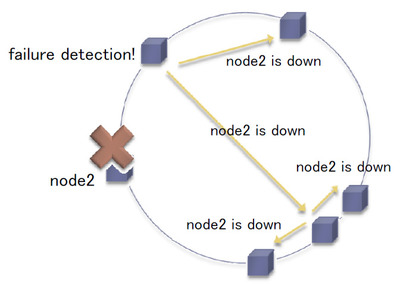
\includegraphics[width=0.5\textwidth]{background/figures/gossip}
    \caption{Gossiping about group membership. A node discovers \texttt{node2} is down, then relays this information to those in his neighbor list.}
    \label{fig:gossip}
\end{figure}


\end{itemize}

\subsection{Failures}
\label{sec:failures}
As we can see, these highly distributed systems are built to allow for failure. We will here explore how Voldemort and Dynamo try to mitigate for failing nodes while also keeping with the operational requirements for consistency and durability. 

\subsubsection{Hinted handoff}
In practice, both nodes and network will fail. During such failures, we still want to continue serving requests.
To satisfy durability during failure, Voldemort perform a form of sloppy quorum. 
Instead of requiring all N members of the quorum to fulfill a durable write, they use temporary hosts. 
By this, we mean that in practice, the N nodes in the preference list a write eventually has to reach, are the next N \emph{healthy} nodes on the ring.
When a node on the preference list is down (marked as not healthy), the request is routed to the next healthy node. 
This write however contains meta data that says who was the intended target for this replica. 
The metadata is then used to push the write back to the intended target once he becomes healthy again.

Looking at Figure \ref{fig:voldemort_hashring}, if a key K hashes to partition 0, the preference list contains nodes \texttt{N0} and \texttt{N1} (recall N=2).
If \texttt{N1} is not responsive, it is not healthy, and assume \texttt{N2} is the next healthy node.
This means that when \texttt{N1} is not responsive, \texttt{N2} is placed on the preference list, because it is the next \emph{healthy} node.
Now when \texttt{N0} receives a write, it will push the replica (to satisfy durability N=2) to \texttt{N2} as long as \texttt{N1} is down.
\texttt{N2} will however receive a write with a hint that this object actually belongs to \texttt{N1}, so \texttt{N2} puts it in a special database to push it to \texttt{N1} at a later time when \texttt{N1} is healthy again. When \texttt{N2} successfully reaches \texttt{N1} and delivers the write, this object is deleted from \texttt{N2}. 
This process is called hinted handoff. 

Using hinted handoff, we can still satisfy durability guarantees during node failures.

\subsubsection{More failures}
Hinted handoff helps in environments with low churn and where nodes usually come back online. But if a node holding a hinted replica goes down before the intended node comes back up, it may even be permanently down and the hinted object is never returned to the intended owner.

To mitigate such permanent failures, Dynamo\cite{dynamo} employs a method to regularly ensure that datasets common between nodes are consistent. A naive approach to this could be sending your entire key set to the other node and compare the data directly.
This is however very costly, both in bandwidth used and is both CPU and disk intensive for both.

To minimize the impact on network load and node performance while simultaneously doing replica synchronization, the database uses hashes of the data. Here Voldemort and Dynamo have different approaches. In Voldemort, each key's hash is sent to the other node for comparison.

In Dynamo, Amazon have implemented merkle trees for comparing data sets between nodes. This significantly reduces workload on a replica synchronization.
A merkle tree is a binary tree of hashes, see Figure \ref{fig:merkletree}, where the leaf nodes are hashes of the key objects.
Now make a hash of the two children nodes.
Then to make the parent node, assign the parent the hash of the two hashes of the children until you have the root node. 

Each node keeps a merkle tree for the keyspace that it shares with the other node. The tree is updated whenever a write is commited.
When a sync happens between two nodes, they only need to compare the value of their root node to know if they have any differences.
One can also see how this method makes it quick to discover which key differs. Each comparison will halve the search area.
I.e. we have a binary search for the differing key or even subtree.

\begin{figure}[h]
    \centering
    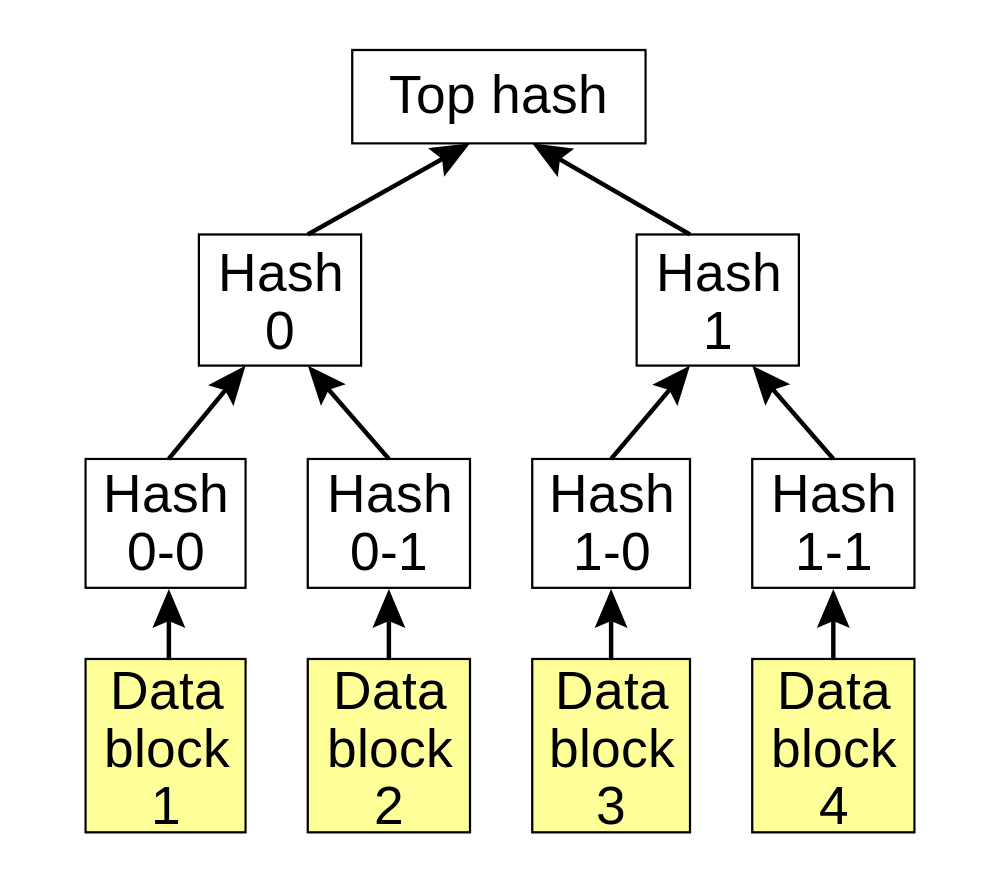
\includegraphics[width=0.5\textwidth]{background/figures/hashtree}
    \caption{Structure of a merkle tree. Notice how the root node can be used for comparing two trees, and how the tree can be used for identifying divergent data.}
    \label{fig:merkletree}
\end{figure}

\subsection{Tunability}
\label{sec:tunability}
As we have briefly outlined above, the database system has three different parameters that are key to operation.
The system gives the admin the opportunity to fine tune certain trade offs after what the implementation needs.

Internally, these are called N, R, W and controls certain aspects of the quorum that is involved in data operations. N is the \emph{eventual} replication factor.
This is the number of nodes we want to store replicas for a key on, and is allowed to happen asynchronously.

\emph{W} is the write factor. This is the number of nodes that synchronously has to be part when we accept a write, and heavily affects performance. 
Typically W is set to two, to make sure an object put must have two replicas in the quorum to be considered successful. 

Another interesting application is the highly writable property store we get with W=1. This means we would never reject a write as long as there is at least one node that can process a request. This will however jeopardize the durability of the data between returning the write and moving the object to other replicas. This setup also has a tendency to introduce a lot more inconsistencies in the data\cite{dynamo}.

The parameter R controls how many nodes must be involved in a read for it to be successful. Setting R low (R=1) would give a high performance read engine. With R=1 though, we might end up with many inconsistencies in the data. It is the read quorum that must decide what data to return. During a read multiple versions of an object might occur. The quorum must then reconcile their versions and return the lastest, or return the conflicting ones.
Because of this, discovering conflicts might be slower when only one node is involved in a read. We are in other words relying on only this single node's world view of the data in a optimistically consistent environment.

Knowing this, when executing a write, the first node to receive the put takes on the role as a coordinator for the write. The coordinator generates the new vector clock and writes a local copy. The coordinator then forwards the request to the top N healthy nodes in the preference list. Nodes that are not healthy are skipped. If W-1 of the healthy nodes report a successful write, the coordinator can return a successful request. 

Reads are handled similarly. The first node receiving the request take on the role as coordinator. The coordinator sends the request to his top N other healthy nodes for the key. After R replies, the coordinator returns the latest version this quorum can agree upon. If there are any divergently versioned objects, all of them are returned to the client for reconciliation.

Amazon\cite{dynamo} mention that their most used configuration for Dynamo is a N=3, W=2, R=2 setup.

\subsection{PAXOS}
Whenever you have a distributed system where errors occur and messages get lost, even simple tasks like deciding on a value can become troublesome. PAXOS is a consensus algorithm made to solve this issue. 

Say we have a set of processes that all can propose values. (The value could be related to leader election). Paxos ensures that a single one of these values is chosen and that all processes involved is notified of this value. If no value is being proposed, then no value should be chosen. 

In Paxos a process can act in three different roles: {\it proposer, acceptor and learner}. A process is not limited to one role at the time. Processes communicate with one another by messages. These messages follow the non-Byzantine model and can take arbitrary long time to be delivered, or they can be lost entirely. They can also be duplicated, however they can not be corrupted. A process acting in a role might also crash, but we assume some critical information will remain through a restart. 

When acting as a proposer, a process will propose a value to a majority subset of acceptors. These acceptors will then accept or deny the proposal according to some rules. Finally if a value is chosen, then all the learners will be informed of this value. The process of choosing a value is given below:

\begin{enumerate}

\item A proposer sends a prepare for proposal message to a majority set of acceptors with a number $n$. This number acts as a timestamp, and represents the last(newest) message this proposer has seen. 
\item Each acceptor receiving this prepare for proposal message will compare the proposed number $n$ with their own highest observed $n$. If the proposed number is higher, then a promise of not accepting any proposal lower than $n$ will be sent back to the proposer along with the acceptors highest observed value. If the proposers number is lower than the acceptors observed number, then the value is sent back along with the highest observed $n$.
\item If the proposer receives a promise from a majority of acceptors, it will send an accept message to the acceptors with the number $n$ along with the value $v$, which is the maximum values received from the acceptors. If the number of promises is less than the majority of acceptors then the attempt has failed, and the proposer must start again with a higher number $n$.
\item When a acceptor receives an accept message, this acceptor will accept this proposal as long as there has not been issued a new proposal with a higher number in the meantime. 
\item Finally, when an acceptor has accepted a proposal it informs all learners. Either by sending a message to all learners, or by sending a message to a designated learner, which in time will inform all other learners. This second step reduces message load but is less reliable.

\end{enumerate}

It is possible to construct a scenario where two proposers keep out proposing each other and no progress is ever made. To combat this a distinguished proposer must be elected. 

Paxos can typically be used in distributed systems to coordinate processes. One example is leader election, another is deciding on the next action to be taken.



\clearpage

\section{Related work}
In this section we will cover Cassandra and HBase. Two other distributed systems that are used 

\subsection{Cassandra}
Cassandra scalable NoSQL database now available as open source through the Apache foundation. It was built from scratch with goal of being a massively scalable NoSQL database. In a cluster running Cassandra there is no sense of a master node, and all communication between nodes use peer to peer and the gossip protocol. As an administrator it is easy to scale Cassandra to meet both current and future system requirements. 

\subsubsection{Reads and writes}
In Cassandra all participating nodes can be accessed for writes and reads. To ensure durability all writes are preceded by a write to a commit log. If a node has crashed, a node holding a replica will service reads and writes according to the hinted handoff strategy. As with Voldemort, Cassandra also features tunable consistency. 

\subsubsection{Data model}
The Cassandra data model is based on a key:value model, however Cassandra extends this model with up to two levels of nesting. This forms a map structure called columns where the outer row key acts as a primary key and the inner sorted map holds all information: \texttt{Map<RowKey, SortedMap<ColumnKey, ColumnValue>>}. By using maps we achieve easy lookups and range scans. By using one more level of nesting we can group columns. These are called super columns. In Cassandra de-normalization is used to be able to efficiently perform queries that accesses information stored in separate columns. To allow this composite columns can be created to match the need of one or more specific queries. These composite columns simply gather information already stored in various columns for easier access. 

\begin{figure}[h]
    \centering
    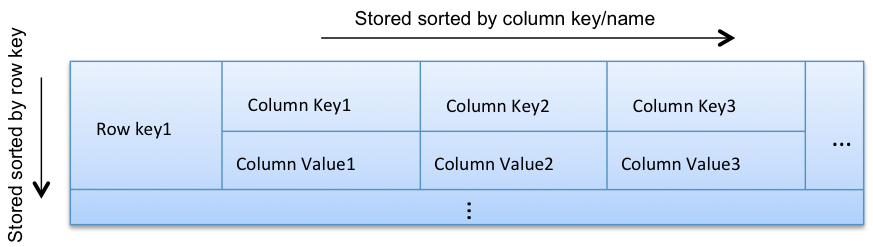
\includegraphics[width=0.5\textwidth]{resources/cas_col.png}
    \caption{A sample column. The row key acts as a primary key and each key:value pair would hold one field in a table. Images borrowed from www.ebaytechblog.com}
    \label{fig:sample_col}
\end{figure}

\begin{figure}[h]
    \centering
    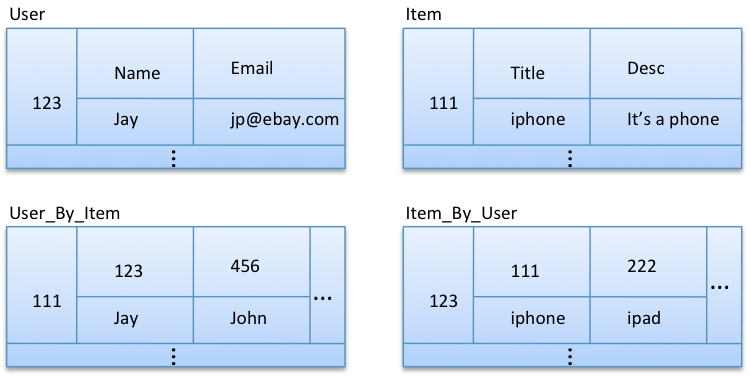
\includegraphics[width=0.6\textwidth]{resources/cas_comp_col.png}
    \caption{A sample composite columns. Here we have separate composite column to efficiently be able to serve queries on users by item and item by users.}
    \label{fig:sample_comp_col}
\end{figure}

\begin{figure}[ht]
	\centering
	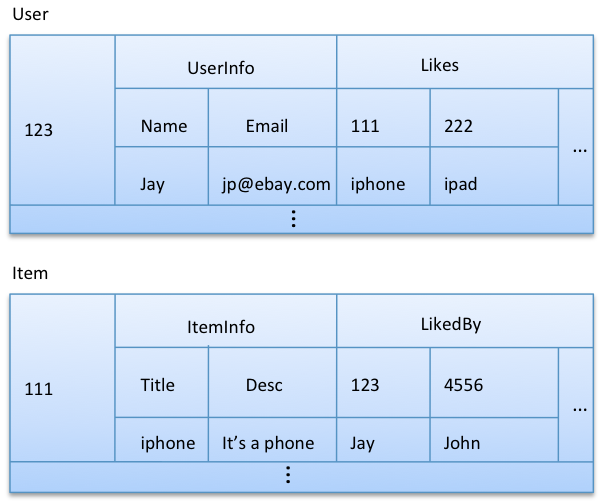
\includegraphics[width=0.4\textwidth]{resources/cas_super_col.png}
	\caption{A sample super column. Here we can see an outer map containing a person and the inner maps consisting of various composite columns}
	\label{fig:sample_super_col}
\end{figure}

Cassandra is used by several well known companies. Netflix uses Cassandra for several applications, including its subscriber system and viewer history service. Facebook used Cassandra to power their inbox search, however this was abandoned in late 2010 in favor of HBase. Spotify also migrated to Cassandra after migrating away from postgreSQL because of scaling issues. They use Cassandra to store playlists, radio stations and notification notifications.

\subsection{HBase}
HBase is based on Googles paper on BigTable.
It is a sparse, distributed, persistent multi-dimensional sorted map.

With regards to the CAP-theorem (Consistency, Availability, Partitioning), HBase provides consistency and tolerance to partitioning, making HBase fault tolerant and easy to reason with in practice.

Important to note is that HBase provides a sparse multi-dimensional \emph{sorted} map.
Keys in the table are sorted, such that similar items are close to another when scanning a table.

E.g. when storing data about urls, the keys are written in reverse: \texttt{com.google.www/users}. This scheme keeps urls from the same domain and subdomain close to each other in the sorted map.

The \emph{rows} or \emph{entries} are typically sparse, meaning that most of the columns, in the table are empty.

To visualize a HBase record, it can help to think of a map of maps:

\begin{lstlisting}
{
	"com.google.www/account": {
		"family": {
			"special": "value"
		},
		"anchor": {
			"com.cnn.www": "value"
		}
	}
	"com.google.www/users": {
		"family": {
			"": "value"
		},
		"anchor": {
			"no.nrk.www": "value"
		}
	}
}
\end{lstlisting}

The families for a record is static for the table at creation, but every family can hold any number of columns within, even many or none.
This is where the sparse property comes from, as most entries will not have a value for the set of all sub-families in the table, leaving most column values empty.

Every \emph{row} or \emph{entry} also has an associated timestamp, used for versioning. This is typically a monotonically increasing number, such as seconds since \emph{epoch}. HBase stores a given number of versions of an entry, and can be queried for these. 
These different versions are stored in descending order, such that the highest number entry, i.e. the newest, is the first entry.

This gives a possible query structure as such \texttt{<key, family:column, timestamp>}. Timestamp is optional. If no timestamp is given, the newest entry is returned. 
If the query has a timestamp, the record with version equal to or less than the given timestamp is returned. If there is no such record, null is returned.

I.e. if we have a query \texttt{<no.nrk.www, referrals:no.nrkbeta.www, 999>}, and we have records in the database:
\begin{lstlisting}
<no.nrk.www, referrals:no.nrkbeta.www, 1001>
<no.nrk.www, referrals:no.nrkbeta.www, 777>
\end{lstlisting}
\texttt{<no.nrk.www, referrals:no.nrkbeta.www, 777>} will be returned.

\subsection{Bone dry servey that explains performance}

\subsection{Netflix Priam for Cassandra}

\subsection{Autoscaling Cassandra clusters}

Baakind\cite{baakind} created a system, called Hecuba, for automatic expansion of Cassandra clusters.

The goal of the project is an automatic scaler for Cassandra. The scaler should based on resource usage be able to increase or decrease the cluster size, based on resource usage in each node of the cluster.
The scaler should not affect the performance of Cassandra. This includes the overall operational capacity for the cluster, as well as only executing scaling when the cluster can handle it, i.e. during times of lower load.

Hecuba includes a master service, which collects information from all the nodes in the cluster, and tries to keep a view of the current status. The Cassandra nodes periodically sends status reports to the master, e.g. one every second. The status report includes size of database, CPU load and memory usage. The master is configured with certain parameters for what loads are allowed, such as maximum memory and CPU load over \emph{a given period of time}.

Like Netflix' Priam, Hecuba does scaling if a threshold is broken for a given period of time. Let's assume a CPU load of 60\%, threshold 55\%, and a period of 10 seconds. Hecuba will then only scale if the CPU load is reported as greater than \emph{threshold} for at least 10 seconds in a row.


\clearpage

\section{There and back again}
\label{sec:prequel}
In this section we will try to shed some light on the preliminary work that was done before we ended up on the path that lead to our project. It will consists of two parts. The first one will be a summary on our pre-project and the second one on our early work with Voldemort.

\subsection{Energy efficiency of a Raspberry Pi cluster used for searching}
Our pre-project was split into three parts. Building a cluster of Raspberry Pis, building a search engine and then measure performance and power efficiency of our cluster compared to a Core i5 Macbook Pro. During the build we constructed our own power supply and built the frame holding the cluster along with network equipment. The search engine was written in C to be as fast as possible. We used an existing python program to create an index over a corpus of text documents, and used tf-idf for scoring results. Through our performance testing we found that even though the Pis require a lot less energy to run, they are unable to keep up with modern hardware in a task so CPU demanding. It is worth mentioning that our entire index fit into memory, so a more disk bound application could have seen very different results. We however feel this is unlikely, due to the disk controller on the PI being very slow and USB based with no DMA, so it requires CPU cycles to do any operation.

\begin{figure}[h]
    \centering
    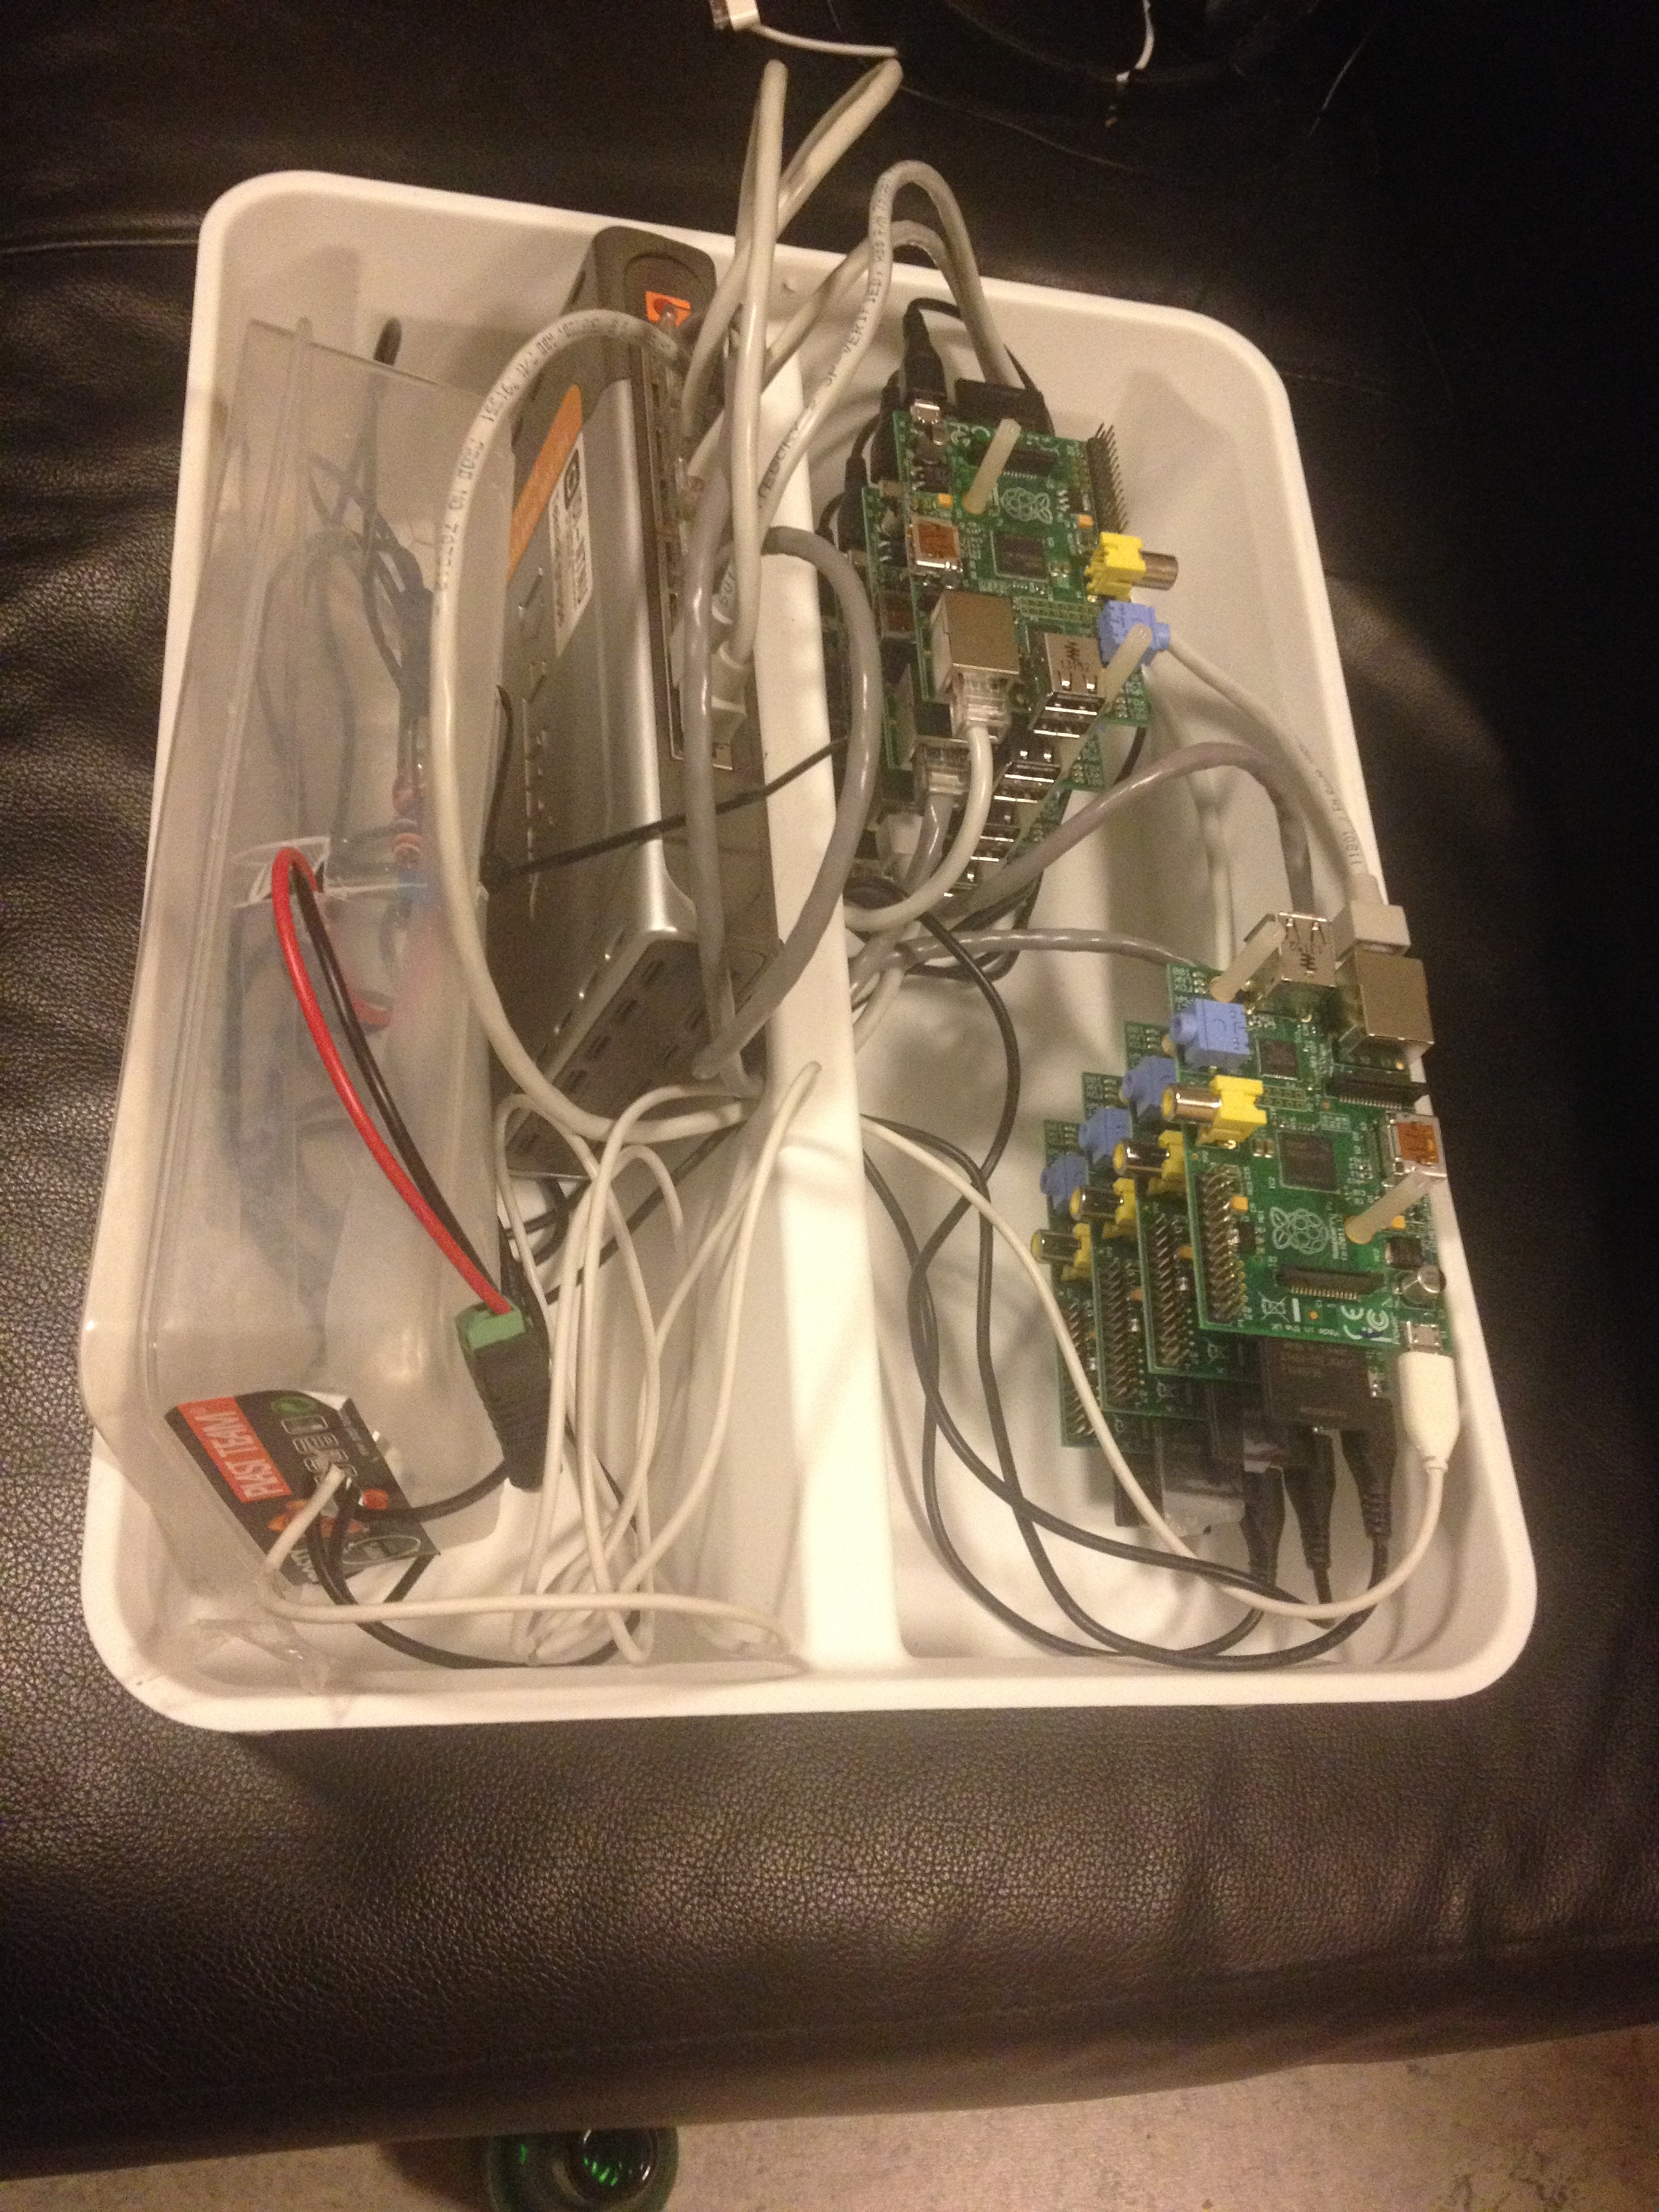
\includegraphics[width=0.5\textwidth]{thereandbackagain/cluster_beautiful.jpg}
    \caption{The Raspberry Pi cluster}
    \label{fig:cluster}
\end{figure}

\subsection{Early work with Raspberry Pis and Voldemort}
In the early days of our project we were planning to use our Raspberry Pi cluster to host a Voldemort service. However the limited memory of 512MB quickly turned out to be a problem. The Pis could run Voldemort without any problems until some of the background data exchange processes started and killed the JVM. After some debugging we determined that memory was a serious issue, and abandoned the idea of running Voldemort on our Pis. They do not have enough RAM for any practical uses of the software.

To try out how much more powerful hardware you need to run a cluster based on Voldemort, we decided to give virtual machines a try. We used an older Mac mini (mid 2010) with a 2.4 Ghz Core 2 Duo processor and 8 GB of RAM, and created 4 virtual machines using VMware Fusion. They were all setup to run Arch Linux with 1 GB memory allocated. Initial tests quickly showed that these had no issues with running out of memory. After querying the institute for a proper solution we were allowed access to 4 virtual machines running on a server within the institute. These servers were running on a Intel(R) Xeon(R) CPU E5-2650 @ 2.00GHz host, with each VM granted 1 GB RAM. The network to these machines were however clogged by several 100mbit links, so we could not get much performance from them, and decided to work more locally.

\subsection{Post mortem}
In our pre-project we built a search engine and ran it on a cluster composed of 8 Raspberry PIs. In this project we wanted to work with a more developed distributed system and explore what possibilities existed for further work, but the typical software packages was unable to run reliably on a small system like the PI. The main problem was the OS running out of memory.
We have chosen to work with Voldemort, which is an open source implementation of Amazon’s Dynamo. This is a highly available NoSQL database that can be run on several nodes. The system is however a bit cumbersome to setup and especially maintain.
As clusters grow in size, management and administrative tasks can become increasingly complex, so we have decided to focus our work on automation and management of a working cluster of nodes running Voldemort. 

\clearpage

\section{Setup}
\label{sec:setup}

To be able to utilize the distributed part of Voldemort it was nessesary to 

\subsection{Begrepsavklaring}
A \texttt{write} or \texttt{put} in the context of ZooKeeper is considered a ZooKeeper \texttt{setData} operation.

A ZooKeeper event, is an event triggered by a watch set in ZooKeeper, giving push information about a change in ZooKeeper about a znode being watched.

In the context of ZooKeeper, the word file might be used for a znode. File used in the context of a local filesystem is a local file.

\subsection{Cluster Setup}
IDI VMS:  Intel(R) Xeon(R) CPU E5-2650 0 @ 2.00GHz, 1 gb ram per instance


\clearpage


\clearpage
\section{Apache ZooKeeper}
We have relied heavily on ZooKeeper in order to store our Voldemort configuration data as well as handling coordination in Headmaster. In this section we will explain what ZooKeeper is along with how it works. Finally we will present which techniques we have used along with how we used them. 

\subsection{What is ZooKeeper}
From Apache ZooKeepers own website\cite{zookeeper} they explain ZooKeeper as:

\blockquote{ZooKeeper is a centralized service for maintaining configuration information, naming, providing distributed synchronization, and providing group services. All of these kinds of services are used in some form or another by distributed applications.}

ZooKeeper offers a simple yet powerful set of services. When designing ZooKeeper they decided not to implement specific primitives server side and instead exposing an API allowing application developers to create their own primitives. This allows for ZooKeeper to be adapted to suit the requirements of different applications, instead of constraining developers to a fixed set of primitives. 

\subsection{Znodes}
ZooKeeper behaves almost like a file system with one key difference. Instead of files and directories - we have znodes. These znodes can contain information in the form of text. One znodes can have children which again can have more children. Together they form an hierarchical structure. 

Znodes also include version numbers for data changes, ACL changes and timestamps to allow cache validations as well as coordinate updates. Whenever a znode's data is change, it's version number increases. This is also true for whenever a client receives data. 

\begin{figure}[h]
    \centering
    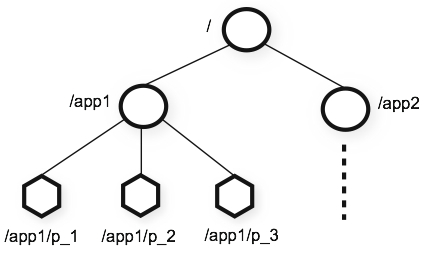
\includegraphics[width=0.4\textwidth]{software/zknamespace.jpg}
    \caption{A sample namespace}
    \label{fig:zk_namespace}
\end{figure}

These znodes can have different flags set which control their behavior. These are persistent, ephemeral and sequential. Persistent is self explanatory. When this flag is set during a put operation, the data will remain in ZooKeeper even though the client disconnects. Ephemeral is the opposite. Data placed in ZooKeeper with this flag will be deleted when the client loses its session. If sequential is set to be true then each child of the znode will have a monotonic increasing sequence number appended to its path. This number is relative to the parent znode, so children znodes can have equal or different names. Ephemeral and sequential are powerful features which enable us to utilize ZooKeeper for leader election, coordination as well as locks. 

\subsection{ZooKeeper Guarantees}
ZooKeeper provides two basic ordering guarantees:

\begin{itemize}
	\item Asynchronous linearizable writes
 	\item FIFO client order
\end{itemize}

Since we have asynchronous writes a client can have several outstanding operations, but ZooKeeper guarantees that they will be executed in FIFO order. ZooKeeper also provides clients with the option to listen for changes on a znode. ZooKeeper guarantees that a client will receive a changeEvent before see the new state of the system following the change. 

\subsection{Watches}
As mentioned above, a client can request a watch on a znode in ZooKeeper. This watch will give the client a changeEvent the next time this znode changes. These changes includes changes in number of children, change in data of znode or that the znode has been deleted. These watches can also be put on non existing znodes which gives the client an event when the znode is registered in ZooKeeper. It is however important to note that a watch will only trigger once, and it is not possible to request infinite watches. So it is up to each individual client to request a new watch after receiving an event.

Because of ZooKeepers linearizable guarantees a read following one of these watchEvents will always return the new state of the system. In the event of several changes in quick succession it is possible for a client to not be notified of each individual change. It will however always be able to determine the final state of the system after all the changes.

\subsection{Implementation}

As mentioned ZooKeeper can be used for more than just storing configuration data. In this section we will explain some different ways to use ZooKeeper with short psudo code examples. 

\subsubsection{Group membership}
ZooKeeper can be used to keep track of group membership. To do this we create a znode for the group at a given path. Now members can register their membership by creating a child znode with the ephemeral flag set. As long as they have a session with ZooKeeper they will be listed as a member of the group. When a member registers as a child they also put a watch on the parent node. If there is a change in membership, for example a node is added, then all nodes set to watch for changes will receive an event. Because of ZooKeepers FIFO ordering guarantees we will never have the case that a node is added some existing node is not notified. 

\subsubsection{Leader election}
Leader election is something that frequently needs to be addressed in a distributed system. In our own Headmaster client we used ZooKeeper to handle this issue. 

To elect a leader we utilize the sequential and ephemeral flags of a znode. We have a znode called leaders in ZooKeeper where potential leaders can register themselves. This znode has the sequential flag set so we get a total order on the potential leaders. We also force each potential leader to use the ephemeral flag when registering. This ensures that when a client disconnects it is removed from the leader znode.By default the znode with the lowest sequence number will be the one that is the leader.

If a potential leader does not win the election (I.E: There is another contender with a lower sequence number) it puts a watch on the winner and waits for changes. If eventually the leader disconnects then there will once again be elected a new leader based on sequence number.

Any client wanting to get a hold of its leader can simply ask ZooKeeper for all the children of the leader znode, and then determine which one is the leader based on sequence numbers. Now the client can put a watch on this leader znode and be notified whenever there is a change in leadership. If said event is received the client simply ask ZooKeeper again for the children and repeat the process.

\subsubsection{Locks}
Another typical use case for ZooKeeper is handling locks. The way we implement locks is by having a reserved path for a znode called lock in ZooKeeper. To control the lock a client must be the one to create this znode with the ephemeral flag set. We use ephemeral to prevent a client for keeping the lock forever in case of a disconnect. 

Any client wanting to use the resource related to the lock will try to create the lock znode. On success that client have access to the resource while in case of a failure the client will put a watch on the lock and wait for the existing znode to be deleted before trying to create it again.

It is also possible to separate locks into read and write locks. In ZooKeeper their only difference will be in the naming of the znode, but the client now can regard them as read or write locks. The case explained above is a typical write lock. In the case of a read lock, the client will be allowed access to the resource as long as there is no write locks before it. If there is a write lock ahead of the read the client will put a watch on said lock and wait until it is deleted. 






 

\clearpage

% implementation.tex

Our work and implementation happened mainly in 3 parts. Part 1 consists of integrating ZooKeeper support and mechanisms into a Voldemort server. Making Voldemort read configurations and storing data in ZooKeeper. Part 2 contains our work towards rebalancing by the help of ZooKeeper. In Part 3 we create the service Headmaster, which is a process to run along side of the Voldemort process. Headmaster listens to active nodes in the cluster, and can generate configuration for new nodes, add them to the cluster, and prepare the members for a rebalance to include the new node. Lastly we have included a part (\ref{sec:testing}) about how we validated our implementation while working.


\section{Part 1}
Integrating ZooKeeper into Voldemort and taking advantage of the coordination services ZooKeeper provides, proved rather difficult.
We chose to override and rewrite much of the current MetadataStore implementation to one that uses ZooKeeper as the backend storage engine instead of local files. 
Actual data is still of course stored locally, but configuration (meta data) now resides in the ZooKeeper cluster.
This abstraction works rather well for shared data files, but causes some issues with information that is stored for individual nodes. 
As such, we landed on a fixed path scheme, where certain configuration files are expected to reside on known locations, and will be presented later.

This change introduces the dependency of a running ZooKeeper cluster for normal operation of any node. While this is a liability and potential source for downtime in a highly available system, ZooKeeper is itself a highly available system and the 5 node setup is regarded as very stable and in heavy use at Yahoo\cite{need:citation}.
TODO: CITATION

Alternatively we could have made the coordination service optional, but we then considered it risky to allow updating config files live through ZooKeeper. In any case, the system will in general be able to operate through short ZooKeeper outages, as all meta and config data is cached locally, however changes will not propagate to the affected nodes as quickly.

\subsection{Configuration}
Configuration is stored in a VoldemortConfig object. Normally this is created from settings stored in local files per node. At startup, the code looks for a properties file in a directory given by environment variable \texttt{VOLDEMORT\_HOME}. 

Now, if you specify a ZooKeeper connection URL as a command line parameter, the program looks for configuration in ZooKeeper.
We have given an example outline of the expected directory structure in Figure \ref{fig:configdirs}. This is for the three nodes \texttt{vold0.idi.ntnu.no}, \texttt{vold1.idi.ntnu.no} and \texttt{vold2.idi.ntnu.no}. You can see the expected path follows the pattern \texttt{/config/HOSTNAME/server.properties}. 

The startup code then reads the config file and tries to parse. If parsing fails, the server is set to fail to clearly signal something is wrong at startup, and needs immediate fixing. If the file is not found, the server registers a watch on the path in ZooKeeper. If there is a write to this file, ZooKeeper will let the server know and the config file can be re-read. 

One can argue whether to fail or listen when a config is not found, but we decided for the latter, to listen for changes, after implementing the management service. As we later will see, listening allows us to push new config files to a node by the help of our management daemon Headmaster. 

\begin{figure}[h]
\dirtree{%
.1 / \ldots{} \begin{minipage}[t]{8cm}(root directory)
			  \end{minipage}.
.2 config.
.3 nodes \ldots{} (individual node configs).
.4 vold0.idi.ntnu.no \ldots{} (hostname).
.5 server.properties.
.5 server.state.
.5 node.id.
.4 vold1.idi.ntnu.no.
.5 server.properties.
.5 server.state.
.5 node.id.
}
\caption{Individual node configs in the shared space.}
\label{fig:configdirs}
\end{figure}

Our modification inherits from the original VoldemortConfig object, so that the ZooKeeper capable version can be used in the same code, in the same manner. The modified code reads data from a fixed location in ZooKeeper, and sets the necessary settings and properties for the server to boot and join the cluster. The ZooKeeper connection URL is passed as a command line parameter.

The directory structure for the whole program can be viewed in its entirety in Figure \ref{fig:dirstruct}, and has been included for completeness.

\begin{figure}[h]
\dirtree{%
.1 / \ldots{} \begin{minipage}[t]{8cm}(The root can also be a chroot{.})
			  \end{minipage}.
.2 active .
.3 vold0.idi.ntnu.no \ldots{} (ephemeral).
.3 vold2.idi.ntnu.no \ldots{} (ephemeral).
.2 config \ldots{} (persistent) . 
.3 nodes (individual node configs).
.4 vold0.idi.ntnu.no.
.5 server.properties.
.5 server.state.
.5 node.id.
.4 vold1.idi.ntnu.no.
.5 server.properties.
.5 server.state.
.5 node.id.
.4 vold2.idi.ntnu.no.
.5 server.properties.
.5 server.state.
.5 node.id.
.3 cluster.xml.
.3 stores.xml.
.2 headmaster.
.3 headmaster\_0009 \ldots{} (ephemeral \& sequential).
.3 headmaster\_0011 \ldots{} (ephemeral \& sequential).
.3 headmaster\_0012 \ldots{} (ephemeral \& sequential) .
}
\caption{Directory structure in ZooKeeper. The nodes or directories are actually Znodes and can hold data.}
\label{fig:dirstruct}
\end{figure}

\subsection{MetadataStore}
The internal state for a node is written to a \texttt{Store} called \texttt{MetadataStore}. It consists of an in memory cache store, and a persistent one to disk. The different stores are implementations of an abstract data \texttt{Store}. As such, we wrote a \texttt{Store} using ZooKeeper as the backend, and used this for persistent storage.

At startup we read the global configuration, the cluster and stores settings, from the Store. The Store fetches the requested files from ZooKeeper, and leaves a watch on the nodes. Because a store \emph{only} \emph{stores} data, the Store itself can not take advantage of the event deliveries from ZooKeeper: The Store keeps no application logic, and can be thought of as a hash map.

To notify and update the internal state of the node on events, we found it necessary to receive events in the configuration management logic, written in the \texttt{MetadataStore}.

When an event from the ZooKeeper client is delivered to the \texttt{MetadataStore}, we first sort it by type.
If it is a management event, like a disconnect event, we temporarily disable the ZooKeeper backend and serve data from the cache until it is reconnected. In our testing, such disconnects (session expiry) happened about once every hour, but the reconnect was usually done in less than two seconds. This instability may be due to our ZooKeeper cluster consisting of a single node and being on a different network.

After a session expiry, we receive a reconnected event when the ZooKeeper client reestablishes a connection. At this point, all set watches are lost, and all events during the connection loss will have been lost. We must therefore reset all watches and check the global configuration data on reconnect. 

\section{Handling the ZooKeeper connection}
Our handling of the ZooKeeper client and connection went through many stages and changes as we got a better understanding of its features.

Our currently preferred design can be viewed in \texttt{ActiveNodeZKListener}.
The ActiveNodeZKListener class wraps a ZooKeeper client connection, providing event delivery to the interface \texttt{ZKDataListener}. 
This approach removes a lot of the noise generated by the client, and delivers clear events that are simpler and clearer to handle and reason with when coding application logic.

We provide the following listener events:
\begin{description}

	\item[dataChanged(path):] 
		This method is called when data has been written to the watched Znode on \texttt{path}.
	\item[nodeDeleted(path):] 
		A call to the listener to let it know the Znode on \texttt{path} has been deleted.
	\item[reconnected():] 
		The connection handler provides a simple call \texttt{reconnected()} when a connection is reestablished after session expiry. When this call happens, we know it is safe to do sanity checking of our state and register watches again.
	\item[childrenList(path):]
		This one is a little bit special. This method is called whenever a Znode's children list is changed. Recall that Znodes are like nodes in a tree, and can have many children. This method call indicates new or removed children for the node on \texttt{path}.

\end{description}

We also include the possibility for receiving the raw events from the ZooKeeper client in the interface:

\begin{description}
	\item[process(event):]
		\texttt{Event} is the raw WatchedEvent from the ZooKeeper client. Registering as a \texttt{Watcher} will forward every internal ZooKeeper event to the listener.

\end{description}




\section{Part 2}

\subsection{Initial configuration}


\subsection{Rebalance}
Another issue we bumped into is related to the architecture of Voldemort.
In a rebalance, the new config files are pushed (written) to each node separately using Voldemort admin data requests. This causes every node to execute a put of the new data on the MetadataStore.

As explained above, we use ZooKeeper for (persistently) sharing the global configuration files.
Also, we would like to be notified about changes to the config files using watches. So first you have N nodes in the cluster, executing N writes to the same file. Each file write potentially triggers N watches, causing a read and watch reset. Worst case we will end up with N writes and N*N watch triggers and reads, all in quick succession (less than a second).
We therefore decided to ignore such put requests in the ZooKeeper driven persistent Store, and only put the new data in the Metadata cache store, deferring the admin to use a ZooKeeper write operation to put the new config out, making the nodes do a re-read.


\subsection{Begrepsavklaring}
A \texttt{write} or \texttt{put} in the context of ZooKeeper is considered a ZooKeeper \texttt{setData} operation.

A ZooKeeper event, is an event triggered by a watch set in ZooKeeper, giving push information about a change in ZooKeeper about a znode being watched.

In the context of ZooKeeper, the word file might be used for a znode. File used in the context of a local filesystem is a local file.

\section{Part 4}
\label{sec:testing}
TODO: Tests and unit tests?
When working on large projects, a lot of code lines are involved. To prevent breaking functionality underway, and to help verify correct (desired) behavior while working, we decided to write unit tests. 
Because of the complex series of events that need to happen while running the program to execute your desired code, it is much easier and more efficient to test and verify your code programmatically in a test environment. The design and verification of our Headmaster program greatly benefited from this approach. The event chain to test the code can be fairly complex, even though the application logic is fairly straight forward.

To create a test environment, we used JUnit and the Mockito project to mimic the behavior we need for validation.
Mockito is a testing framework for Java. It allows to create ``mock'' objects that can be used to trigger and verify program behavior in a predictable and controlled manner. The ``fake'', but controllable objects are very useful for eliminating outer dependencies, and instead having them behave in a completely predictable and controlled way.

Listing \ref{lst:mockito} shows a short example of how Mockito and JUnit is used to write short, simple yet powerful functional tests that verify behavior. It is also worth noting that the resulting test code is quite readable by a programmer.

\begin{lstlisting}[style=customjava,label=lst:mockito,caption={Test code utilizing Mockito. Think of the \texttt{@Mock} class as a subclass with all methods overrided \texttt{return null;}.}]
$$@Mock
ActiveNodeZKListener activeNodeZKListener;

Headmaster headmaster;

public void whenDataChangedTestIfWatchIsReset() {
    String path = "/config/cluster.xml";

    when(activeNodeZKListener.getStringFromZooKeeper(
    	path, true)).thenReturn(EXAMPLE_CLUSTER);

    headmaster.setZKListener(activeNodeZKListener);

    headmaster.dataChanged(path);

    /** 
     * verify method is called with params path, and watch flag set to true.
     */
    verify(activeNodeZKListener, times(1)).getStringFromZooKeeper(path, true);
}

\end{lstlisting}

Here we are verifying that upon receiving a notification that a znode has changed, the Znode (path) is fetched with a new watch set.
All without actually providing a working third party object (ActiveNodeZKListener) to the test, the object is entirely faked with the static \texttt{when} and \texttt{thenReturn} methods. After setting the dependency class up with the desired behavior, it is injected into the class we are testing, then verify that the desired method is called once and only once (\texttt{times(1)}). Similarly it is easy to see how you can verify two calls (\texttt{times(2)}). For zero calls, it is recommended to use the more readable method \texttt{never}.

\clearpage


\section{Headmaster}
Headmaster is our take on managing the cluster.

It is implemented as a standalone service so that it can be run remotely, and independently from Voldemort.
We later decided to move it closer, so that we could keep better uptime on the service and reduce the chance of conflicts.
At one point we had inadvertently started two Headmasters, which kept fighting for control.
We spent a fair amount of time debugging weird race conditions until we realized there was two services listening.

It is now a master based service with leader election through ZooKeeper that can run on any number of nodes.

\clearpage

\clearpage

\section{Hardware}
\label{sec:hardware}

\subsection{Mac Mini}
We server running voldemort is a a Mac Mini Mid 2010 model. It has a Intel Core Duo 2.4 GHz processor, 8 GBs of RAM and solid state storage. We run the latest OS X 10.9.1

\begin{figure}[h]
    \centering
    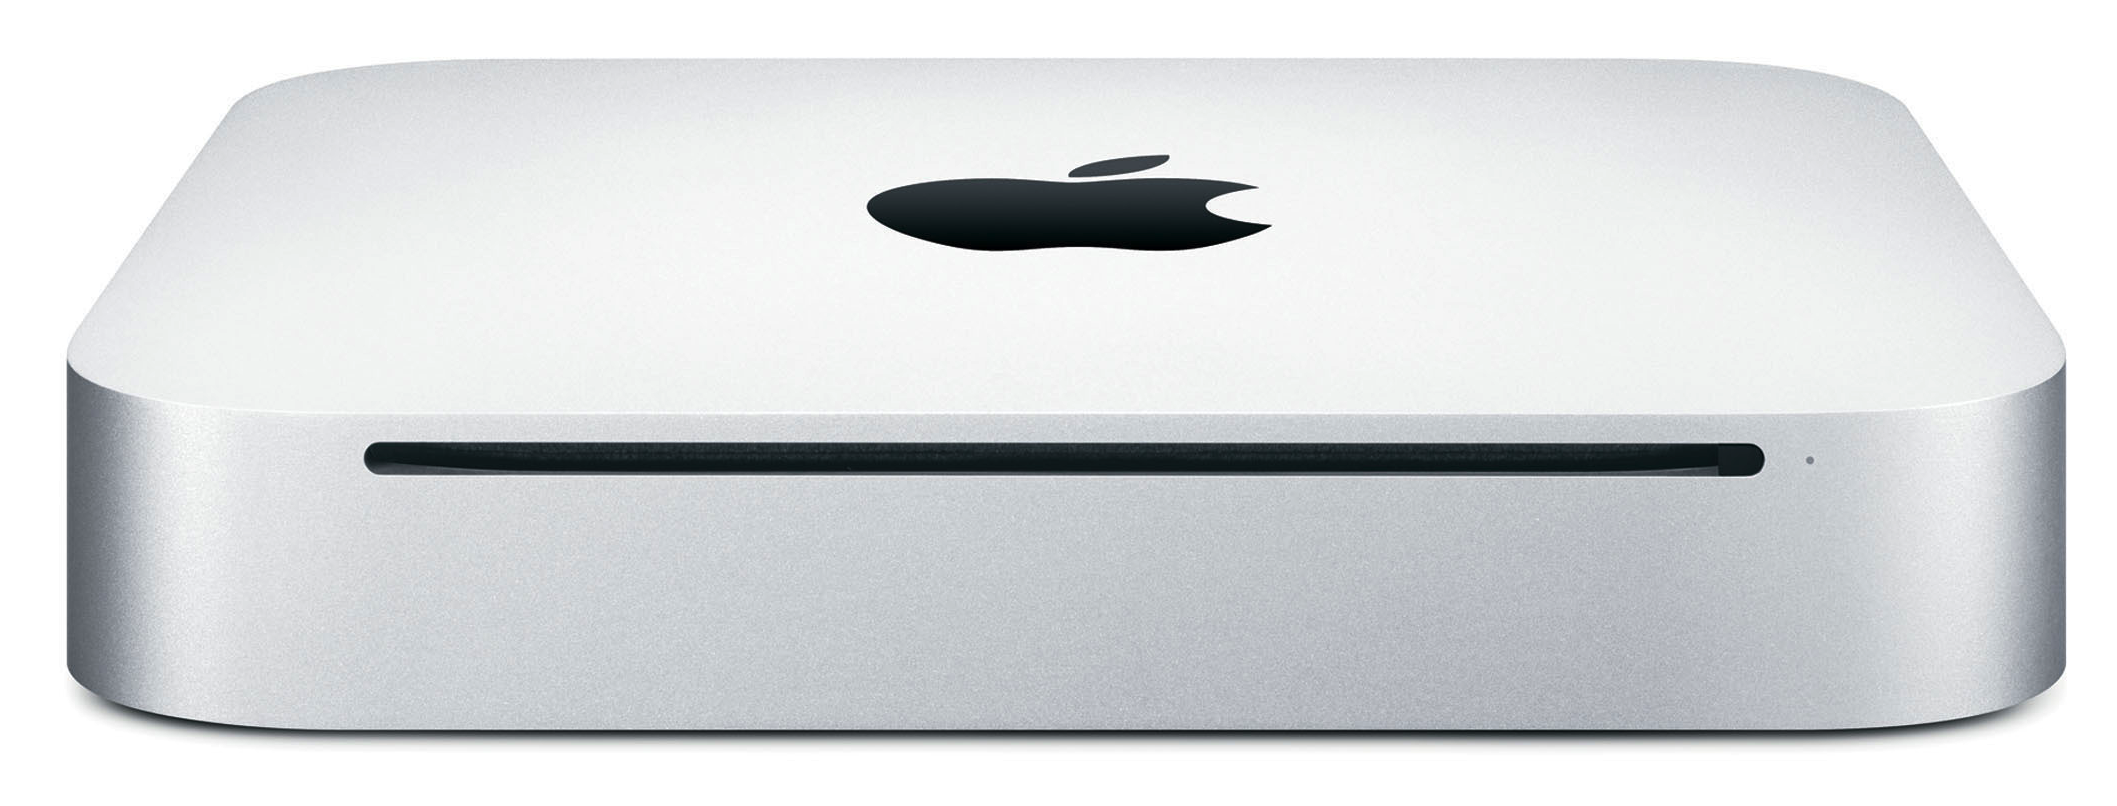
\includegraphics[width=0.8\textwidth]{hardware/mac-mini-06-2010}
    \caption{Mac Mini 2010}
    \label{fig:macmini_hw}
\end{figure}


\clearpage

\bibliographystyle{plain}
\bibliography{references}

\end{document}
